\documentclass[beamer]{standalone}

\begin{document}
\section{Introduzione}
\subsection{Presentazione del dataset}
\begin{frame}
\frametitle{\secname : \subsecname}
Il dataset consiste di osservazioni in archi temporali variabili dell'accelerazione $\vec{a} = \begin{pmatrix}
a_x \\ a_y \\ a_z
\end{pmatrix}$ a cui il cellulare è sottoposto.
\end{frame}

\begin{frame}

\begin{columns}[T] % align columns
\begin{column}{.48\textwidth}
\begin{figure}[H]
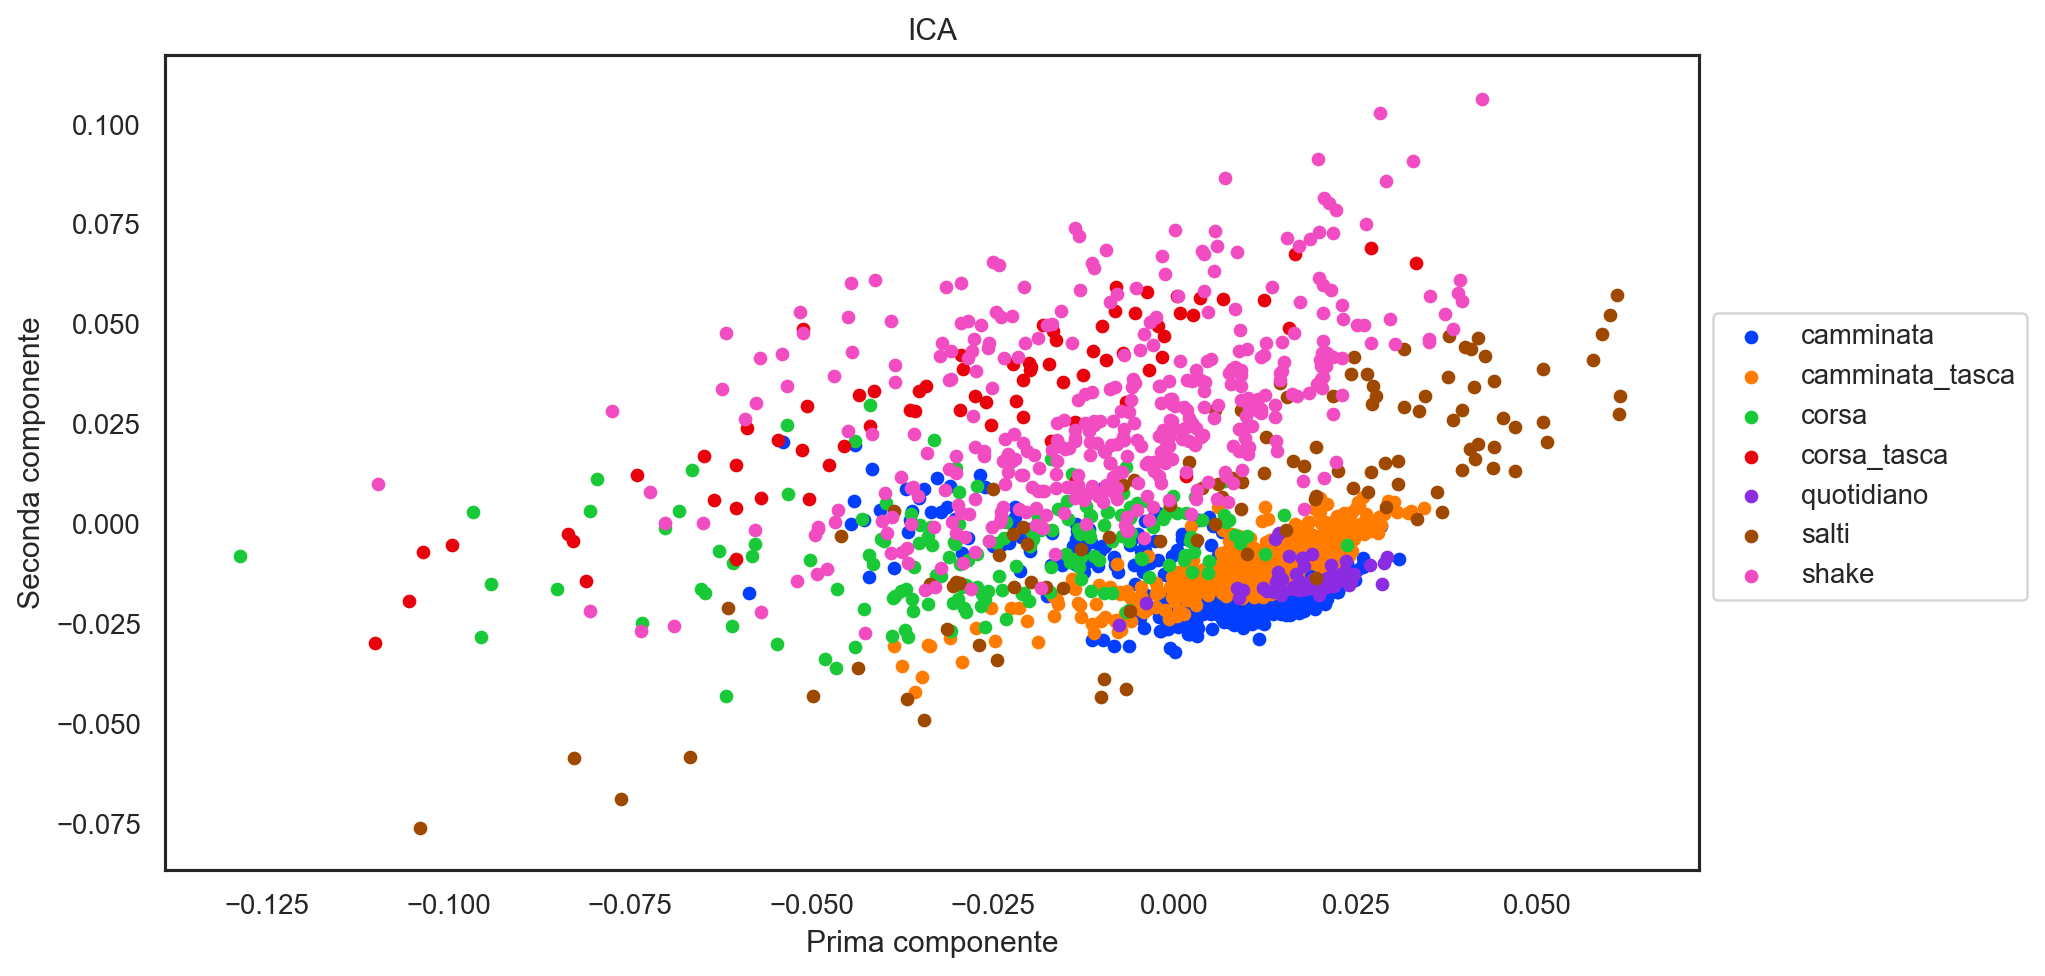
\includegraphics[width=\textwidth]{../figure/ICA.png}
\end{figure}
\end{column}%
\hfill%
\begin{column}{.48\textwidth}
$f(x)=x^2$
\end{column}%
\end{columns}
\end{frame}


\end{document}